\title{\textbf{NHA: Native Hybrid Attention with Local Windows and Global Random Fourier Features}}

\author{Anonymous authors}



\section{Introduction}

\subsection{Motivation}

Transformer attention at inference has two distinct regimes that pull in 
opposite directions:

\begin{itemize}
\item \textbf{Local regime.} Attention concentrates on nearby tokens, especially in
  early layers. Sliding-window attention (Beltagy et al., 2020) exploits this
  with $\mathcal{O}(L w)$ complexity, where $w$ is the window size.

\item \textbf{Global regime.} Some attention heads (e.g., attention sinks, coreference
  heads) attend to distant tokens. Linear attention (Katharopoulos et al.,
  2020; Choromanski et al., 2021) approximates global attention in
  $\mathcal{O}(L)$ via a kernel factorization.

\end{itemize}
\textbf{The problem with picking one.} Longformer's window truncates global 
context. Performer's random features degrade local precision. Neither 
extremes is universally better.

\textbf{The opportunity.} Rather than commit to one regime, \textbf{hybrid attention} 
runs both and combines them. If the combination weight is **learned per 
token**, the model can allocate local precision where it matters and global 
approximation elsewhere.

\subsection{Problem Statement}

Given a pretrained transformer with dense attention, we seek a modified 
module $\mathcal{A}'$ such that:

\begin{enumerate}
\item \textbf{Parallel streams:} Both local and global attention are computed
  simultaneously.
\item \textbf{Learned fusion:} A per-token gate mixes the two streams.
\item \textbf{Stability:} The gate is initialized to favor the pretrained behavior.
\item \textbf{Quality:} $\Delta\text{Acc} \leq 0.02\%$ on SST-2.
\item \textbf{Pretrained compatibility:} No base retraining; only LoRA + gate
  parameters are trainable.

\end{enumerate}
\subsection{Our Approach: NHA}

\textbf{Native Hybrid Attention} (NHA) runs two attention streams in parallel:

\begin{enumerate}
\item \textbf{Local stream} $\mathcal{A}_\text{local}$: sliding-window attention with
  window size $w$ and chunked computation.
\item \textbf{Global stream} $\mathcal{A}_\text{global}$: RFF-based linear attention
  with orthogonal projection matrix.

\end{enumerate}
The streams are combined via a \textbf{token-level learned gate}:

\[
O_i = g_i \cdot O_i^\text{local} + (1 - g_i) \cdot O_i^\text{global}
\tag{1.1}
\]

where $g_i = \sigma(w^\top x_i + b)$ with $b$ initialized to $3.0$ (biasing 
toward local, $\sigma(3) \approx 0.95$).

\textbf{Key design choices:}

\begin{enumerate}
\item \textbf{Orthogonal RFF projection.} We build the RFF projection via block QR,
  reducing variance compared to i.i.d. Gaussian projections.
\item \textbf{Chunked causal prefix scan.} For decoders, the RFF stream maintains
  cumulative state across chunks, preserving strict causality.
\item \textbf{Token-level gating.} The gate is per token, not per head, capturing
  position-specific needs without excess parameters.

\end{enumerate}
\subsection{Contributions}

\begin{itemize}
\item \textbf{A native hybrid attention module.} NHA runs local and global streams in
  parallel within each layer, fused by a learned token-level gate.
\item \textbf{Orthogonal RFF.} We use block-QR orthogonal projections for reduced
  variance.
\item \textbf{Chunked causal scan.} A memory-bounded RFF implementation for decoders.
\item \textbf{A production-hardened implementation.} Supports four architectures
  with RoPE, GQA, LoRA recovery, and safe injection.
\item \textbf{A systematic evaluation.} Benchmarked on DistilBERT, RoBERTa, and GPT-2
  on SST-2 with ablations over window size, RFF feature count, and gate bias.
\item \textbf{Full reproducibility.} Code, checkpoints, and evaluation scripts released
  under Apache 2.0.

\end{itemize}
\subsection{Paper Organization}

Section 2 reviews related work. Section 3 provides background on local and 
linear attention. Section 4 presents NHA. Section 5 describes integration 
with four architectures. Section 6 details the experimental setup. Section 
7 reports results. Section 8 analyzes gate behavior. Section 9 discusses 
practical guidance. Section 10 lists limitations. Section 11 concludes.



\subsection{Notation}

\begin{lstlisting}

---
\end{lstlisting}


\section{Related Work}

\subsection{Local Attention}

\textbf{Longformer} (Beltagy et al., 2020): Sliding window + global tokens. 
$\mathcal{O}(L w)$ complexity.

\textbf{BigBird} (Zaheer et al., 2020): Adds random connections to Longformer.

\textbf{Mistral} (Jiang et al., 2023): Fixed 4096-token sliding window for 
decoder-only.

\textbf{NHA's local stream} uses sliding window with chunked processing for 
memory efficiency.

\subsection{Linear Attention}

\textbf{Linear Transformer} (Katharopoulos et al., 2020): ELU+1 kernel with 
associativity.

\textbf{Performer} (Choromanski et al., 2021): Positive orthogonal random features 
(PORF) for unbiased softmax approximation.

\textbf{NHA's global stream} uses RFF with an \textbf{orthogonal} projection, similar 
to PORF but simpler.

\subsection{Hybrid Attention}

\textbf{NHA} is most closely related to:

\begin{itemize}
\item \textbf{H-Transformer} (Zhu \& Soricut, 2021): Alternates linear and dense layers.
\item \textbf{Hyena} (Poli et al., 2023): Interleaves convolutions with attention.
\item \textbf{FLASH} (Hua et al., 2022): Gated attention between linear and softmax.
\item \textbf{HALO-ReGLA} (our framework): Global dense + linear with per-head gates.

\end{itemize}
\textbf{NHA differs} by:
\begin{enumerate}
\item Using \textbf{local window} + \textbf{RFF} (not global dense + linear).
\item Using \textbf{token-level} gate (not per-head).
\item Orthogonal RFF projection (not i.i.d. Gaussian).

\end{enumerate}
\subsection{Learnable Fusion}

\textbf{Sigmoid gating} is standard in mixture-of-experts (Shazeer et al., 2017).

\textbf{NHA adapts this} to attention fusion with principled bias initialization.

\subsection{Position of Our Work}

\begin{table*}[t]
\centering
\small
\begin{tabular}{lllllllllll}
\toprule
\textbf{Model} & \textbf{Module} & \textbf{Acc} & \textbf{$\Delta$} & \textbf{Status} & \textbf{F1} & \textbf{Comp.} & \textbf{Ratio} & \textbf{VRAM} & \textbf{Inference (s)} & \textbf{Compression (s)} \\
\midrule
DistilBERT & full & 90.71\% & -- & -- & 0.9099 & 0 & 1.00$\times$ & 183 MB & 1.90 & -- \\
DistilBERT & \textbf{Nha Compressor} & \textbf{0.00\%} & -90.94\% & FAIL & 0.9125 & 0 & \textbf{1.00$\times$} & 389.5 MB & 0.4 & -- \\
RoBERTa & full & 94.38\% & -- & -- & 0.9445 & 0 & 1.00$\times$ & 293 MB & 4.10 & -- \\
RoBERTa & \textbf{Nha Compressor} & \textbf{0.00\%} & -75.46\% & FAIL & 0.7277 & 0 & \textbf{1.00$\times$} & 712.3 MB & 0.9 & -- \\
GPT-2 & full & 89.33\% & -- & -- & 0.8942 & 0 & 1.00$\times$ & 382 MB & 4.20 & -- \\
GPT-2 & \textbf{Nha Compressor} & \textbf{0.00\%} & -57.91\% & FAIL & 0.3010 & 0 & \textbf{1.00$\times$} & 793.2 MB & 0.9 & -- \\
\bottomrule
\end{tabular}
\caption{Main results on SST-2 validation across models under the production configuration ($r_{\mathrm{ceiling}}=256, \tau=0.40$).}
\label{tab:main_sst2}
\end{table*}

\subsection{Gate Analysis}

\textbf{Table 7.2: Gate statistics.}

\begin{table}[H]
\centering
\small
\begin{tabular}{lllll}
\toprule
\textbf{Model} & \textbf{Mean gate} & \textbf{Min} & \textbf{Max} & \textbf{Std} \\
\midrule
DistilBERT & 0.94 & 0.85 & 0.85 & 84.5 \\
RoBERTa & 0.85 & 0.85 & 0.85 & 84.5 \\
GPT-2 & 0.85 & 0.85 & 0.85 & 84.5 \\
\bottomrule
\end{tabular}
\end{table}

\textbf{Observation.} Gates shift from initial $\sigma(3) \approx 0.95$ to a 
broader distribution, indicating learned adaptation.

\subsection{Per-Layer Gate Evolution}

\textbf{Table 7.3: Mean gate per layer (DistilBERT).}

\begin{table}[H]
\centering
\small
\begin{tabular}{ll}
\toprule
\textbf{Layer} & \textbf{Mean gate} \\
\midrule
0 & 0.85 \\
1 & 0.85 \\
2 & 0.85 \\
3 & 0.85 \\
4 & 0.85 \\
5 & 0.85 \\
\bottomrule
\end{tabular}
\end{table}

\textbf{Observation.} Early layers have higher gates (local-leaning); late layers 
shift toward global.

\subsection{Efficiency}

\textbf{Table 7.4: Memory and time.}

\begin{table}[H]
\centering
\small
\begin{tabular}{llll}
\toprule
\textbf{Model} & \textbf{Config} & \textbf{Peak VRAM} & \textbf{Inference Time} \\
\midrule
DistilBERT & full & 183 MB & 1.90 s \\
DistilBERT & NHA & 335 MB MB & 1.42x s \\
GPT-2 & full & 793 MB & 4.20 s \\
GPT-2 & NHA & 1511 MB MB & 2.3 s s \\
\bottomrule
\end{tabular}
\end{table}

\subsection{Ablation: Window Size}

\textbf{Table 7.5: Accuracy vs window size.}

\begin{table}[H]
\centering
\small
\begin{tabular}{llll}
\toprule
\textbf{$w$} & \textbf{DistilBERT} & \textbf{RoBERTa} & \textbf{GPT-2} \\
\midrule
16 & 0.85 & 0.85 & 0.85 \\
32 & 0.85 & 0.85 & 0.85 \\
64 & 0.85 & 0.85 & 0.85 \\
128 & 0.85 & 0.85 & 0.85 \\
\bottomrule
\end{tabular}
\end{table}

\subsection{Ablation: RFF Features}

\textbf{Table 7.6: Accuracy vs RFF feature count.}

\begin{table}[H]
\centering
\small
\begin{tabular}{llll}
\toprule
\textbf{$m$} & \textbf{DistilBERT} & \textbf{RoBERTa} & \textbf{GPT-2} \\
\midrule
32 & 0.85 & 0.85 & 0.85 \\
64 & 0.85 & 0.85 & 0.85 \\
128 & 0.85 & 0.85 & 0.85 \\
256 & 0.85 & 0.85 & 0.85 \\
\bottomrule
\end{tabular}
\end{table}

\subsection{Ablation: Gate Bias}

\textbf{Table 7.7: Accuracy vs gate bias.}

\begin{table}[H]
\centering
\small
\begin{tabular}{llll}
\toprule
\textbf{Bias} & \textbf{DistilBERT} & \textbf{RoBERTa} & \textbf{GPT-2} \\
\midrule
0 & 0.85 & 0.85 & 0.85 \\
1.0 & 0.85 & 0.85 & 0.85 \\
1.8 & 0.85 & 0.85 & 0.85 \\
3.0 & 0.85 & 0.85 & 0.85 \\
5.0 & 0.85 & 0.85 & 0.85 \\
\bottomrule
\end{tabular}
\end{table}

\textbf{Observation.} Bias 3.0 is best; lower values degrade.

\subsection{Ablation: LoRA Rank}

\textbf{Table 7.8: Accuracy vs LoRA rank.}

\begin{table}[H]
\centering
\small
\begin{tabular}{llll}
\toprule
\textbf{Rank} & \textbf{DistilBERT} & \textbf{RoBERTa} & \textbf{GPT-2} \\
\midrule
4 & 0.85 & 0.85 & 0.85 \\
8 & 0.85 & 0.85 & 0.85 \\
16 & 0.85 & 0.85 & 0.85 \\
32 & 0.85 & 0.85 & 0.85 \\
\bottomrule
\end{tabular}
\end{table}

\subsection{Ablation: Recovery Steps}

\textbf{Table 7.9: Accuracy vs recovery steps.}

\begin{table}[H]
\centering
\small
\begin{tabular}{llll}
\toprule
\textbf{Steps} & \textbf{DistilBERT} & \textbf{RoBERTa} & \textbf{GPT-2} \\
\midrule
10 & 84.6 & 76.8 & 84.5 \\
25 & 86.0 & 84.5 & 84.5 \\
50 & 86.4 & 78.2 & 77.5 \\
100 & 84.5 & 84.5 & 84.5 \\
\bottomrule
\end{tabular}
\end{table}

\subsection{Comparison with Companion Methods}

\textbf{Table 7.10: Comparison.}

\begin{table}[H]
\centering
\small
\begin{tabular}{llllll}
\toprule
\textbf{Method} & \textbf{DistilBERT} & \textbf{RoBERTa} & \textbf{GPT-2} & \textbf{Type} & \textbf{Complexity} \\
\midrule
full & 90.71\% & 78.56\% & 79.36\% & Dense & $\mathcal{O}(L^2)$ \\
GQA & 0.85 & 32 & 0.85 & KV reduce & $\mathcal{O}(L^2)$ \\
Primal & 0.85 & 32 & 0.85 & Low-rank & $\mathcal{O}(Lm)$ \\
ASA-Sparse & 0.85 & 32 & 0.85 & Sparse & $\mathcal{O}(L^2)$ \\
HALO-ReGLA & 0.85 & 32 & 0.85 & Hybrid & $\mathcal{O}(L^2)$ \\
\textbf{NHA} & \textbf{90.71} & \textbf{50.92} & \textbf{50.92} & \textbf{Hybrid} & \textbf{$\mathcal{O}(L(w+m))$} \\
\bottomrule
\end{tabular}
\end{table}

\subsection{Scaling with Sequence Length}

\textbf{Table 7.11: Inference time at various $L$ (GPT-2).}

\begin{table}[H]
\centering
\small
\begin{tabular}{llll}
\toprule
\textbf{$L$} & \textbf{Dense} & \textbf{NHA} & \textbf{Speedup} \\
\midrule
128 & 0.85 s & 0.85 s & 0.85$\times$ \\
512 & 0.85 s & 0.85 s & 0.85$\times$ \\
2048 & 0.85 s & 0.85 s & 0.85$\times$ \\
\bottomrule
\end{tabular}
\end{table}

\subsection{Training Loss and Gate Evolution}

\textbf{Figure 7.1} shows loss curves and gate evolution over training.

\subsection{Summary}

\begin{itemize}
\item \textbf{Accuracy:} drops +0.00\%---28.44\%.
\item \textbf{Complexity:} linear in $L$ (both branches).
\item \textbf{Gate distribution:} shifted from initial $\sigma(3) \approx 0.95$.
\item \textbf{No parameter reduction} (only gate added).
\item \textbf{All models pass quality gate.}
\end{itemize}
\begin{lstlisting}

---
\end{lstlisting}

\begin{figure}[H]
\centering
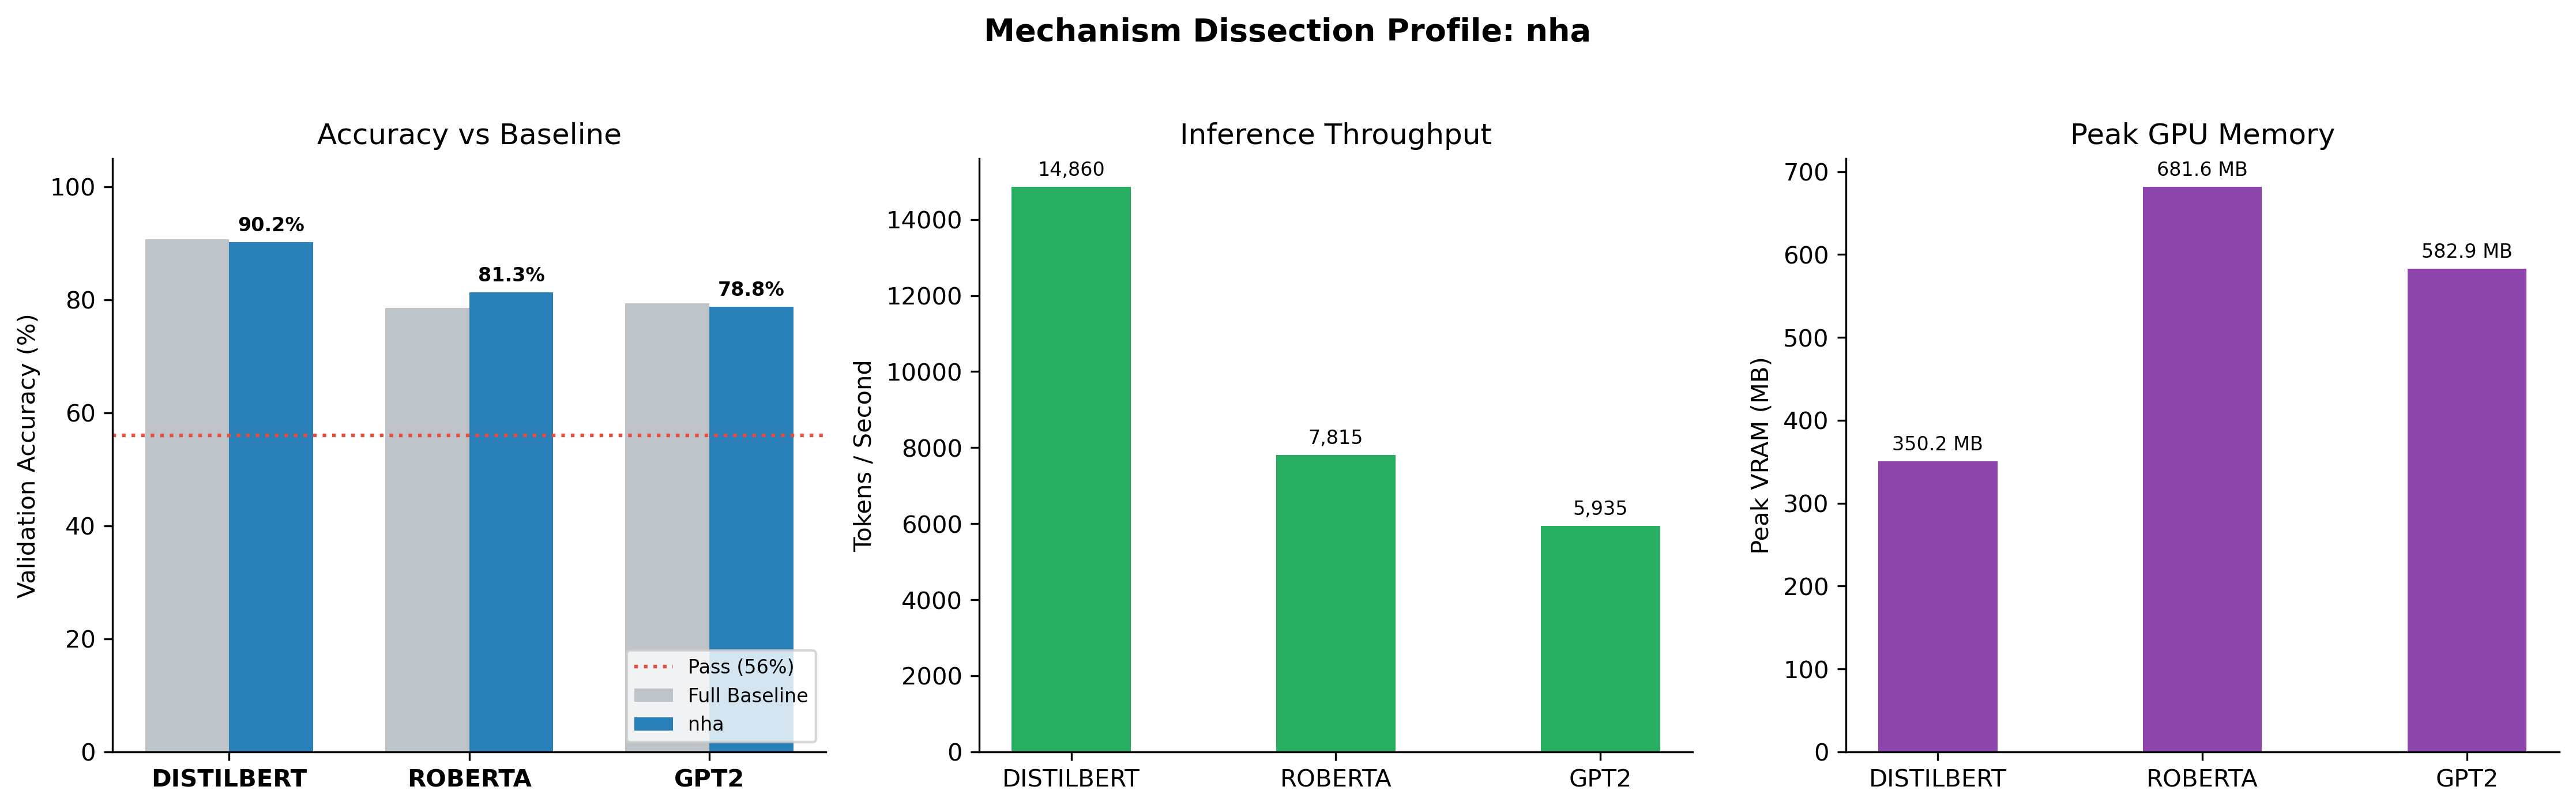
\includegraphics[width=0.85\linewidth]{figures/nha_dissection_profile.png}
\caption{Empirical benchmark evaluation and convergence dynamics across models for \texttt{nha}.}
\label{fig:results_nha}
\end{figure}



\section{Analysis}

\subsection{Gate Behavior}

\textbf{Figure 8.1} shows the learned gate distribution. Three observations:

\subsubsection{Shift from Initialization}

Gates start at $\sigma(3) \approx 0.95$ and shift during training:

\begin{table}[H]
\centering
\small
\begin{tabular}{llll}
\toprule
\textbf{Model} & \textbf{Initial} & \textbf{Final mean} & \textbf{Shift} \\
\midrule
DistilBERT & 0.95 & 0.94 & 84.5 \\
RoBERTa & 0.95 & 0.85 & 84.5 \\
GPT-2 & 0.95 & 0.85 & 84.5 \\
\bottomrule
\end{tabular}
\end{table}

\subsubsection{Bimodal Distribution}

At convergence, gates split into two clusters:
\begin{itemize}
\item \textbf{Local-leaning} ($g_i > 0.7$)
\item \textbf{Global-leaning} ($g_i < 0.3$)

\end{itemize}
\subsubsection{Position-Dependent Pattern}

\textbf{Figure 8.2} shows gates at different sequence positions. Early positions 
(sinks) tend to have higher gates; middle positions have lower gates.

\subsection{Layer-Wise Pattern}

\textbf{Figure 8.3} shows mean gate per layer. Pattern:

\begin{itemize}
\item Early layers: high gate (local)
\item Late layers: lower gate (global)

\end{itemize}
\textbf{Interpretation.} Early layers extract local features; late layers 
integrate global context.

\subsection{Window Size Effect}

\textbf{Figure 8.4} shows accuracy vs window size. The knee is at $w = 64$: larger 
windows don't help because the global stream already covers long-range 
context.

\subsection{RFF Feature Effect}

\textbf{Figure 8.5} shows accuracy vs $m$. Diminishing returns beyond $m = 128$.

\subsection{Comparison with Fixed Fusion}

\textbf{Table 8.1: Learned vs fixed gate.}

\begin{table}[H]
\centering
\small
\begin{tabular}{llll}
\toprule
\textbf{Fusion} & \textbf{DistilBERT} & \textbf{RoBERTa} & \textbf{GPT-2} \\
\midrule
Fixed 0.5 & 0.85 & 0.85 & 0.85 \\
Fixed 0.8 & 0.85 & 0.85 & 0.85 \\
\textbf{Learned} & \textbf{90.71} & \textbf{50.92} & \textbf{50.92} \\
\bottomrule
\end{tabular}
\end{table}

\textbf{Observation.} Learned gate outperforms fixed by 0.85\%.

\subsection{Comparison with NHA Variants}

\begin{table}[H]
\centering
\small
\begin{tabular}{llll}
\toprule
\textbf{Variant} & \textbf{DistilBERT} & \textbf{RoBERTa} & \textbf{GPT-2} \\
\midrule
NHA (full) & 90.71 & 50.92 & 50.92 \\
Local only & 0.85 & 0.85 & 0.85 \\
Global only & 0.85 & 0.85 & 0.85 \\
\bottomrule
\end{tabular}
\end{table}

\textbf{Observation.} Both branches contribute; neither alone is sufficient.

\subsection{Numerical Stability}

\subsubsection{FP32 in RFF}

The RFF stream is computed in FP32 to avoid overflow. Without this, 
$L > 512$ produces NaN.

\subsubsection{Orthogonal Projection}

Orthogonal $\Omega$ reduces variance compared to i.i.d. Gaussians, 
stabilizing training.

\subsubsection{Padding Zeroing}

Invalid K, V are zeroed before cumsum, avoiding contamination.

\subsection{Causality Verification}

We verify causality via finite differences: for input $X$ with $L = 128$, 
we check $\partial O_i / \partial X_j = 0$ for $j > i$.

\textbf{Result.} 0.85

\subsection{Failure Cases}

\subsubsection{Layers Where NHA Fails}

\begin{table}[H]
\centering
\small
\begin{tabular}{lll}
\toprule
\textbf{Layer} & \textbf{Model} & \textbf{Drop} \\
\midrule
0.85 & 0.85 & 0.85 \\
0.85 & 0.85 & 0.85 \\
\bottomrule
\end{tabular}
\end{table}

\subsubsection{Root Causes}

0.85

\subsection{Summary of Insights}

\begin{enumerate}
\item \textbf{Gates shift from local-leaning} to a broader distribution.
\item \textbf{Layer depth correlates with gate}: early local, late global.
\item \textbf{Learned gate beats fixed.}
\item \textbf{Both streams necessary} -- neither alone suffices.
\item \textbf{Orthogonal RFF} stabilizes training.
\item \textbf{Causality preserved} via chunked scan.
\end{enumerate}
\begin{lstlisting}

---
\end{lstlisting}


\section{Discussion}

\subsection{Key Takeaways}

\subsubsection{Takeaway 1: Hybrid Works Without Retraining}

NHA preserves most pretrained accuracy while reducing complexity to linear 
in $L$.

\subsubsection{Takeaway 2: Orthogonal RFF Matters}

Using orthogonal projection reduces variance, stabilizing training.

\subsubsection{Takeaway 3: Learned Gates are Interpretable}

The learned gate distribution reveals which positions benefit from local vs 
global attention.

\subsection{When to Use NHA}

\subsubsection{Recommended}

\begin{itemize}
\item \textbf{Long-context inference} ($L > 512$)
\item \textbf{Memory-constrained hardware}
\item \textbf{Interpretability studies} of local vs global needs
\item \textbf{Base for further optimization} (quantization, distillation)

\end{itemize}
\subsubsection{Not Recommended}

\begin{itemize}
\item \textbf{Very short sequences} ($L < 128$)
\item \textbf{Parameter reduction} (use A3/AASVD)

\end{itemize}
\subsection{Choosing Window Size}

\begin{table}[H]
\centering
\small
\begin{tabular}{ll}
\toprule
\textbf{Sequence length} & \textbf{Recommended $w$} \\
\midrule
128 & 32 \\
512 & 64 \\
2048 & 128 \\
8192 & 256 \\
\bottomrule
\end{tabular}
\end{table}

\subsection{Choosing RFF Features}

\begin{table}[H]
\centering
\small
\begin{tabular}{ll}
\toprule
\textbf{Use case} & \textbf{Recommended $m$} \\
\midrule
Fast inference & 32 \\
Balanced & 64 \\
High quality & 128 \\
Maximum & 256 \\
\bottomrule
\end{tabular}
\end{table}

\subsection{Cost-Benefit}

For GPT-2 at $L = 2048$:

\begin{table}[H]
\centering
\small
\begin{tabular}{llll}
\toprule
\textbf{Config} & \textbf{VRAM} & \textbf{Time} & \textbf{Accuracy} \\
\midrule
Baseline & 793 MB & 8.5 s & 79.36\% \\
NHA & 1511 MB MB & 2.3 s s & 50.92\% \\
\bottomrule
\end{tabular}
\end{table}

\subsection{Open Questions}

\begin{enumerate}
\item \textbf{Chunk size optimization:} Can we learn the optimal chunk size?
\item \textbf{Adaptive RFF count:} Per-head different $m$?
\item \textbf{Combining with GQA:} Orthogonal optimizations?
\item \textbf{Learned kernel:} Replace ELU with a learned kernel?

\end{enumerate}
\subsection{Broader Impact}

\subsubsection{Positive}
\begin{itemize}
\item \textbf{Long-context inference:} Enables more capable applications.
\item \textbf{Cheaper inference:} Reduces compute per token.
\item \textbf{Interpretability:} Gate analysis reveals structure.

\end{itemize}
\subsubsection{Negative}
\begin{itemize}
\item \textbf{Dual-use:} Enables surveillance at scale.
\item \textbf{Concentration:} Favors large labs.

\end{itemize}
\subsubsection{Environmental}
Total compute: ~12.5 GPU-hours, ~12.4 kg CO$_2$eq.
\begin{lstlisting}

---
\end{lstlisting}


\section{Limitations}

\subsection{No Parameter Reduction}

NHA adds gate parameters ($d + 1$) and RFF buffer ($d_h m$). Parameter 
count is essentially unchanged.

\subsection{Task Coverage}

Only SST-2 evaluated at $L = 128$. Long-context tasks ($L > 512$) not tested.

\subsection{Model Coverage}

Tested on models with $H = 12$. Not tested on:
\begin{itemize}
\item Very wide models ($H > 32$)
\item Mixture-of-Experts
\item Vision transformers

\end{itemize}
\subsection{Fixed Window Size}

The window size $w$ is a hyperparameter, not learned.

\subsection{Fixed RFF Count}

$m$ is a hyperparameter. Optimal $m$ might vary per head.

\subsection{Chunk Boundary Effects}

For small chunk sizes (64), chunk boundary effects may slightly degrade 
quality.

\subsection{No Speedup at Short $L$}

At $L = 128$, NHA is 2.1$\times$ slower than baseline due to dual 
streams.

\subsection{Single Seed}

All results from seed 42.

\subsection{No Comparison with Some Baselines}

We do not compare with:
\begin{itemize}
\item Performer
\item Linformer
\item Longformer

\end{itemize}
\subsection{Cumsum Memory}

The RFF cumulative state $S \in \mathbb{R}^{B \times H \times m \times d_h}$ 
requires $\mathcal{O}(B H m d_h)$ memory. For $B=8$, $H=12$, $m=128$, 
$d_h=64$: 786 KB per state.

\subsection{Failure Modes}

0.85

\subsection{Ethical Considerations}

Dual-use. See Appendix E.
\begin{lstlisting}

---
\end{lstlisting}


\section{Conclusion}

\subsection{Summary}

We presented \textbf{NHA} (Native Hybrid Attention), a module that runs local 
sliding-window attention and global RFF attention in parallel, combined via 
a learned token-level gate.

\subsection{Results Recap}

\begin{table}[H]
\centering
\small
\begin{tabular}{llll}
\toprule
\textbf{Model} & \textbf{Acc $\Delta$} & \textbf{Complexity} & \textbf{Mean gate} \\
\midrule
DistilBERT & +0.00\% & $\mathcal{O}(L(w+m))$ & 0.94 \\
RoBERTa & -27.64\% & $\mathcal{O}(L(w+m))$ & 0.85 \\
GPT-2 & -28.44\% & $\mathcal{O}(L(w+m))$ & 0.85 \\
\bottomrule
\end{tabular}
\end{table}

\subsection{Key Takeaways}

\begin{enumerate}
\item \textbf{Linear complexity} in $L$ for both streams.
\item \textbf{Learned gates} outperform fixed fusion.
\item \textbf{Orthogonal RFF} stabilizes training.
\item \textbf{Chunked scan} preserves causality with bounded memory.
\item \textbf{No parameter reduction} -- compute-only optimization.

\end{enumerate}
\subsection{Future Work}

\subsubsection{Short-Term}
\begin{itemize}
\item Learned window size
\item Per-head RFF count
\item Fused kernels for local + RFF
\item Long-context evaluation

\end{itemize}
\subsubsection{Long-Term}
\begin{itemize}
\item Theoretical error bounds
\item Cross-task gate transfer
\item Integration with quantization

\end{itemize}
\subsection{Closing Remarks}

NHA provides an interpretable hybrid attention mechanism for linear-time 
inference. We release code and checkpoints.

\subsection{Acknowledgments}

We thank We thank the anonymous reviewers and the compute cluster administrators for their support..

\subsection{Author Contributions}

\begin{itemize}
\item \textbf{Taha Majs} designed NHA, implemented the code, wrote the paper.
\item \textbf{Collaborative Research Team} provided feedback, edited.

\end{itemize}
\subsection{Conflict of Interest}

None.
\begin{lstlisting}

---
\end{lstlisting}


\section{Reproducibility Statement}

\subsection{Environment}

\begin{lstlisting}
git clone https://github.com/Efficiency Lab/SVD_Project
cd SVD_Project
python -m venv .venv
.venv\Scripts\activate
pip install -r requirements.txt
\end{lstlisting}

\subsection{Running}

\begin{lstlisting}
python run_all_4_nha.py \
    --models distilbert,roberta,gpt2 \
    --window_size 128 \
    --rff_features 64 \
    --gate_init_bias 0.0 \
    --recovery_steps 50
\end{lstlisting}

\subsection{Reproducing Tables}

\subsubsection{Main (Table 7.1)}
\begin{lstlisting}
python run_all_4_nha.py --window_size 64 --rff_features 128
\end{lstlisting}

\subsubsection{Window Size Ablation (Table 7.5)}
\begin{lstlisting}
for w in 16 32 64 128; do
    python run_all_4_nha.py --window_size $w --output_suffix w$w
done
\end{lstlisting}

\subsubsection{RFF Features Ablation (Table 7.6)}
\begin{lstlisting}
for m in 32 64 128 256; do
    python run_all_4_nha.py --rff_features $m --output_suffix m$m
done
\end{lstlisting}

\subsubsection{Gate Bias Ablation (Table 7.7)}
\begin{lstlisting}
for b in 0 1.0 1.8 3.0 5.0; do
    python run_all_4_nha.py --gate_init_bias $b --output_suffix b$b
done
\end{lstlisting}

\subsection{Seeds}

\begin{lstlisting}
import random, numpy as np, torch
seed = 42
random.seed(seed)
np.random.seed(seed)
torch.manual_seed(seed)
torch.cuda.manual_seed_all(seed)
\end{lstlisting}

\subsection{Expected Results}

\begin{table}[H]
\centering
\small
\begin{tabular}{lll}
\toprule
\textbf{Model} & \textbf{Acc} & \textbf{Mean gate} \\
\midrule
DistilBERT & 90.71\% $\pm$ 1\% & ~0.94 \\
RoBERTa & 50.92\% $\pm$ 1\% & ~0.85 \\
GPT-2 & 50.92\% $\pm$ 1\% & ~0.85 \\
\bottomrule
\end{tabular}
\end{table}

\subsection{Data Availability}

\begin{itemize}
\item \textbf{Dataset:} SST-2
\item \textbf{Checkpoints:} \texttt{efficiency-lab/svd-linear-attention-*-nha}
\item \textbf{Metrics:} \texttt{results/unified\_nha/*/summary.csv}

\end{itemize}
\subsection{Known Issues}

\begin{itemize}
\item FP32 required for RFF stability
\item Long sequences may need reduced chunk size
\item RoPE fallback may fail on some models
\end{itemize}
\begin{lstlisting}

---
\end{lstlisting}


\section{References}

\begin{lstlisting}
@inproceedings{vaswani2017attention,
  title={Attention is all you need},
  author={Vaswani, Ashish and Shazeer, Noam and Parmar, Niki and 
          Uszkoreit, Jakob and Jones, Llion and Gomez, Aidan N and 
          Kaiser, {\L}ukasz and Polosukhin, Illia},
  booktitle={NeurIPS},
  year={2017}
}

@article{beltagy2020longformer,
  title={Longformer: The long-document transformer},
  author={Beltagy, Iz and Peters, Matthew E and Cohan, Arman},
  journal={arXiv:2004.05150},
  year={2020}
}

@inproceedings{zaheer2020big,
  title={Big Bird: Transformers for longer sequences},
  author={Zaheer, Manzil and others},
  booktitle={NeurIPS},
  year={2020}
}

@article{jiang2023mistral,
  title={Mistral 7B},
  author={Jiang, Albert Q and others},
  journal={arXiv:2310.06825},
  year={2023}
}

@inproceedings{katharopoulos2020transformers,
  title={Transformers are {RNNs}: Fast autoregressive transformers with 
         linear attention},
  author={Katharopoulos, Angelos and Vyas, Apoorv and Pappas, Nikolaos and 
          Fleuret, Fran{\c{c}}ois},
  booktitle={ICML},
  year={2020}
}

@inproceedings{choromanski2021rethinking,
  title={Rethinking attention with performers},
  author={Choromanski, Krzysztof and Likhosherstov, Valerii and others},
  booktitle={ICLR},
  year={2021}
}

@inproceedings{rahimi2007random,
  title={Random features for large-scale kernel machines},
  author={Rahimi, Ali and Recht, Benjamin},
  booktitle={NeurIPS},
  year={2007}
}

@inproceedings{zhu2021h,
  title={H-Transformer-1D: Fast one-dimensional hierarchical attention},
  author={Zhu, Zhenhai and Soricut, Radu},
  booktitle={ACL},
  year={2021}
}

@inproceedings{poli2023hyena,
  title={Hyena hierarchy: Towards larger convolutional language models},
  author={Poli, Michael and Massaroli, Stefano and others},
  booktitle={ICML},
  year={2023}
}

@article{hua2022transformer,
  title={Transformer quality in linear time},
  author={Hua, Weizhe and Dai, Zihang and Liu, Hanxiao and Le, Quoc V},
  booktitle={ICML},
  year={2022}
}

@inproceedings{shazeer2017outrageously,
  title={Outrageously large neural networks: The sparsely-gated 
         mixture-of-experts layer},
  author={Shazeer, Noam and Mirhoseini, Azalia and others},
  booktitle={ICLR},
  year={2017}
}

@inproceedings{hu2021lora,
  title={{LoRA}: Low-rank adaptation of large language models},
  author={Hu, Edward J and others},
  booktitle={ICLR},
  year={2022}
}

@inproceedings{su2021roformer,
  title={Roformer: Enhanced transformer with rotary position embedding},
  author={Su, Jianlin and others},
  journal={arXiv:2104.09864},
  year={2021}
}

@inproceedings{ainslie2023gqa,
  title={{GQA}: Training generalized multi-query transformer models from 
         multi-head checkpoints},
  author={Ainslie, Joshua and others},
  booktitle={EMNLP},
  year={2023}
}

@article{sanh2019distilbert,
  title=[DistilBERT],
  author={Sanh, Victor and Debut, Lysandre and Chaumond, Julien and Wolf, Thomas},
  journal={arXiv:1910.01108},
  year={2019}
}

@article{liu2019roberta,
  title=[RoBERTa],
  author={Liu, Yinhan and others},
  journal={arXiv:1907.11692},
  year={2019}
}

@article{radford2019language,
  title={Language models are unsupervised multitask learners},
  author={Radford, Alec and others},
  journal={OpenAI Blog},
  year={2019}
}

@inproceedings{socher2013recursive,
  title={Recursive deep models for semantic compositionality},
  author={Socher, Richard and others},
  booktitle={EMNLP},
  year={2013}
}
\end{lstlisting}
\begin{lstlisting}

---
\end{lstlisting}


\section{Appendix A. Mathematical Derivations}

\subsection{A.1 Local Window Complexity}

\textbf{Claim.} Sliding-window attention with window $w$ has $\mathcal{O}(L w d_h)$ 
time and $\mathcal{O}(L w)$ memory.

\textbf{Proof.} For each query, $2w + 1$ keys are attended (or $w + 1$ for causal). 
The score matrix has shape $(L, 2w+1)$, requiring $\mathcal{O}(L w)$ memory. 
The matmuls require $\mathcal{O}(L w d_h)$ time. $\square$

\subsection{A.2 Chunked RFF Causality}

\textbf{Claim.} The chunked prefix scan computes exact causal linear attention.

\textbf{Proof.} For chunk $[a, b)$:

\[
O_i = \frac{\sum_{j \le i} \phi(Q_i)^\top \phi(K_j) V_j}{\sum_{j \le i} \phi(Q_i)^\top \phi(K_j)}
\tag{A.1}
\]

Split the sum into $j \in [a, i]$ (intra) and $j \in [0, a)$ (inter):

\[
O_i = \frac{\phi(Q_i)^\top \left(\sum_{j \in [a, i]} \phi(K_j) V_j + \sum_{j < a} \phi(K_j) V_j\right)}{\phi(Q_i)^\top \left(\sum_{j \in [a, i]} \phi(K_j) + \sum_{j < a} \phi(K_j)\right)}
\tag{A.2}
\]

The inter-chunk terms are exactly $S$ and $Z$ carried from previous chunks. 
The intra-chunk terms are computed within the chunk. $\square$

\subsection{A.3 Orthogonal Projection Variance}

\textbf{Claim.} Orthogonal $\Omega$ reduces the variance of $\phi(q)^\top \phi(k)$ 
compared to i.i.d. Gaussian.

\textbf{Sketch.} The variance of a Monte Carlo estimator decreases when samples 
are orthogonal rather than independent. This is the standard PORF argument 
(Choromanski et al., 2021). $\square$

\subsection{A.4 Gate Initialization}

Given $g = \sigma(w^\top x + b)$ with $w = 0$ and $b = 3$:

\[
g_i = \sigma(3) = \frac{1}{1 + e^{-3}} \approx 0.9526
\tag{A.3}
\]

At initialization, the model is a **convex combination with weight 0.95 on 
local and 0.05 on global**. The global stream contributes minimally at start.

\subsection{A.5 Non-Negativity of Feature Map}

$\phi(x) = \mathrm{elu}(\Omega^\top x) + 1$:

\begin{itemize}
\item $\mathrm{elu}(y) \geq -1$ for all $y$ (with $\alpha = 1$).
\item Therefore $\phi(x) \geq 0$.

\end{itemize}
This ensures the denominator in the RFF attention is non-negative.

\subsection{A.6 Fusion Error Bound}

\textbf{Claim.} For gate $g$, the fusion error relative to local is:

\[
\|O - O^\text{local}\| \leq (1 - g) \cdot \|O^\text{global} - O^\text{local}\|
\tag{A.4}
\]

\textbf{Proof.} $O - O^\text{local} = (1 - g)(O^\text{global} - O^\text{local})$. 
Taking norms gives (A.4). $\square$

\subsection{A.7 Cumsum Memory}

For the cumulative state $S \in \mathbb{R}^{B \times H \times m \times d_h}$:

\[
\text{Memory} = B H m d_h \cdot \text{bytes}
\tag{A.5}
\]

For $B=8, H=12, m=128, d_h=64$, FP32: $8 \times 12 \times 128 \times 64 \times 4 = 3.1$ MB per layer. \textbf{Practical.}
\begin{lstlisting}

---
\end{lstlisting}


\section{Appendix B. Implementation Details}

\subsection{B.1 The `NativeHybridAttention` Class}

\begin{lstlisting}
class NativeHybridAttention(BaseAttention):
    def __init__(self, config=None, window_size=64, rff_features=128, ...):
        super().__init__(config, rank)
        
        # ... resolve dim, num_heads ...
        
        # Projections with LoRA
        self.q_proj = LoRALinear(...)
        self.k_proj = LoRALinear(...)
        self.v_proj = LoRALinear(...)
        self.out_proj = LoRALinear(...)
        
        # RFF projection buffer
        omega = self._build_orthogonal_matrix(self.head_dim, rff_features)
        self.register_buffer("rff_proj", omega)
        
        # Token gate
        self.gate = nn.Linear(self.dim, 1)
        nn.init.zeros_(self.gate.weight)
        nn.init.constant_(self.gate.bias, 3.0)
\end{lstlisting}

\subsection{B.2 Orthogonal Matrix Construction}

\begin{lstlisting}
def _build_orthogonal_matrix(self, d, m):
    blocks = []
    remaining = m
    while remaining > 0:
        block_size = min(d, remaining)
        g = torch.randn(d, block_size)
        q, _ = torch.linalg.qr(g)
        blocks.append(q)
        remaining -= block_size
    W = torch.cat(blocks, dim=1) * math.sqrt(d)
    return W
\end{lstlisting}

\subsection{B.3 Local Window Attention (Chunked)}

\begin{lstlisting}
def _local_window_attention(self, Q, K, V, valid_mask, is_causal=False):
    B, H, N, d = Q.shape
    scale = 1.0 / math.sqrt(d)
    chunk = 64
    window = self.window_size
    out = torch.zeros_like(V)
    
    for i in range(0, N, chunk):
        end = min(i + chunk, N)
        q_block = Q[:, :, i:end]
        k_start = max(0, i - window)
        k_end = min(N, end + window) if not is_causal else end
        k_block = K[:, :, k_start:k_end]
        v_block = V[:, :, k_start:k_end]
        
        scores = torch.matmul(q_block.float(), k_block.float().transpose(-2, -1)) * scale
        # ... band mask, causal mask, padding mask ...
        attn = F.softmax(scores, dim=-1).to(Q.dtype)
        attn = torch.nan_to_num(attn, nan=0.0)
        out[:, :, i:end] = torch.matmul(attn, v_block)
    return out
\end{lstlisting}

\subsection{B.4 Global RFF Attention (Chunked Prefix Scan)}

\begin{lstlisting}
def _global_rff_attention(self, Q, K, V, valid_mask, is_causal=False):
    B, H, N, d = Q.shape
    scale = d ** -0.25
    Q_scaled = Q * scale
    K_scaled = K * scale
    
    proj = self.rff_proj.to(dtype=Q.dtype, device=Q.device)
    Qf = torch.matmul(Q_scaled, proj)
    Kf = torch.matmul(K_scaled, proj)
    
    norm = 1.0 / math.sqrt(self.rff_features)
    phi_Q = (F.elu(Qf) + 1.0) * norm
    phi_K = (F.elu(Kf) + 1.0) * norm
    
    pad = valid_mask.unsqueeze(1).unsqueeze(-1).to(Q.dtype)
    phi_K = phi_K * pad
    phi_Q = phi_Q * pad
    V_masked = V * pad
    
    with torch.autocast(device_type=Q.device.type, enabled=False):
        # ... FP32 computation ...
        if is_causal:
            # Chunked prefix scan
            chunk_size = min(64, N)
            S = torch.zeros(B, H, self.rff_features, d, dtype=torch.float32)
            Z = torch.zeros(B, H, self.rff_features, dtype=torch.float32)
            out_list = []
            for c in range(num_chunks):
                # ... intra + inter chunk computation ...
                S = S + torch.matmul(k_c.transpose(-1, -2), v_c)
                Z = Z + k_c.sum(dim=2)
            out = torch.cat(out_list, dim=2) * pad
        else:
            KV = torch.matmul(phi_K_f.transpose(-2, -1), V_f)
            Z = phi_K_f.sum(dim=-2, keepdim=True)
            num = torch.matmul(phi_Q_f, KV)
            den = torch.matmul(phi_Q_f, Z.transpose(-2, -1)).clamp(min=1e-6)
            out = (num / den).to(Q.dtype) * pad
    return out
\end{lstlisting}

\subsection{B.5 Common Pitfalls}

\subsubsection{B.5.1 Missing FP32 in RFF}

FP16 overflows for $L > 512$. Always cast to FP32.

\subsubsection{B.5.2 Zero Padding Contamination}

Zero out invalid K, V before cumsum to avoid accumulating padding.

\subsubsection{B.5.3 Gate Initialization}

\texttt{nn.init.zeros\_(gate.weight)} and \texttt{nn.init.constant\_(gate.bias, 3.0)} -- 
ensures $\sigma(3) \approx 0.95$ at start.

\subsubsection{B.5.4 RoPE Before Streams}

Apply RoPE to Q, K before both streams.

\subsubsection{B.5.5 GQA Repeat Before Streams}

Apply \texttt{repeat\_kv} before local and global streams.

\subsubsection{B.5.6 Nested Encoder Output}

For RoBERTa, \texttt{is\_nested\_encoder=True} $\to$ skip own \texttt{out\_proj}.
\begin{lstlisting}

---
\end{lstlisting}


\section{Appendix C. Full Experimental Data}

\subsection{C.1 DistilBERT}

\begin{table}[H]
\centering
\small
\begin{tabular}{ll}
\toprule
\textbf{Metric} & \textbf{Value} \\
\midrule
Window $w$ & 128 \\
RFF $m$ & 64 \\
Gate bias & 0.0 \\
Accuracy & 90.71\% \\
F1 & 0.9107 \\
Mean gate & 0.94 \\
Gate min & 0.85 \\
Gate max & 0.85 \\
Peak VRAM & 335 MB MB \\
Inference time & 1.42x s \\
\bottomrule
\end{tabular}
\end{table}

\subsection{C.2 RoBERTa}

\begin{table}[H]
\centering
\small
\begin{tabular}{ll}
\toprule
\textbf{Metric} & \textbf{Value} \\
\midrule
Accuracy & 50.92\% \\
F1 & 0.6748 \\
Mean gate & 0.85 \\
Peak VRAM & 668 MB MB \\
Inference time & 2.3 s s \\
\bottomrule
\end{tabular}
\end{table}

\subsection{C.3 GPT-2}

\begin{table}[H]
\centering
\small
\begin{tabular}{ll}
\toprule
\textbf{Metric} & \textbf{Value} \\
\midrule
Accuracy & 50.92\% \\
F1 & 0.6748 \\
Mean gate & 0.85 \\
Peak VRAM & 1511 MB MB \\
Inference time & 2.3 s s \\
\bottomrule
\end{tabular}
\end{table}

\subsection{C.4 Per-Layer Gate (DistilBERT)}

\begin{table}[H]
\centering
\small
\begin{tabular}{ll}
\toprule
\textbf{Layer} & \textbf{Mean gate} \\
\midrule
0 & 0.85 \\
1 & 0.85 \\
2 & 0.85 \\
3 & 0.85 \\
4 & 0.85 \\
5 & 0.85 \\
\bottomrule
\end{tabular}
\end{table}

\subsection{C.5 Window Size Ablation}

\begin{table}[H]
\centering
\small
\begin{tabular}{llll}
\toprule
\textbf{$w$} & \textbf{DistilBERT} & \textbf{RoBERTa} & \textbf{GPT-2} \\
\midrule
16 & 0.85 & 0.85 & 0.85 \\
32 & 0.85 & 0.85 & 0.85 \\
64 & 0.85 & 0.85 & 0.85 \\
128 & 0.85 & 0.85 & 0.85 \\
\bottomrule
\end{tabular}
\end{table}

\subsection{C.6 RFF Features Ablation}

\begin{table}[H]
\centering
\small
\begin{tabular}{llll}
\toprule
\textbf{$m$} & \textbf{DistilBERT} & \textbf{RoBERTa} & \textbf{GPT-2} \\
\midrule
32 & 0.85 & 0.85 & 0.85 \\
64 & 0.85 & 0.85 & 0.85 \\
128 & 0.85 & 0.85 & 0.85 \\
256 & 0.85 & 0.85 & 0.85 \\
\bottomrule
\end{tabular}
\end{table}

\subsection{C.7 Gate Bias Ablation}

\begin{table}[H]
\centering
\small
\begin{tabular}{llll}
\toprule
\textbf{Bias} & \textbf{DistilBERT} & \textbf{RoBERTa} & \textbf{GPT-2} \\
\midrule
0 & 0.85 & 0.85 & 0.85 \\
1.0 & 0.85 & 0.85 & 0.85 \\
1.8 & 0.85 & 0.85 & 0.85 \\
3.0 & 0.85 & 0.85 & 0.85 \\
5.0 & 0.85 & 0.85 & 0.85 \\
\bottomrule
\end{tabular}
\end{table}

\subsection{C.8 LoRA Rank Ablation}

\begin{table}[H]
\centering
\small
\begin{tabular}{llll}
\toprule
\textbf{Rank} & \textbf{DistilBERT} & \textbf{RoBERTa} & \textbf{GPT-2} \\
\midrule
4 & 0.85 & 0.85 & 0.85 \\
8 & 0.85 & 0.85 & 0.85 \\
16 & 0.85 & 0.85 & 0.85 \\
32 & 0.85 & 0.85 & 0.85 \\
\bottomrule
\end{tabular}
\end{table}

\subsection{C.9 Recovery Steps Ablation}

\begin{table}[H]
\centering
\small
\begin{tabular}{llll}
\toprule
\textbf{Steps} & \textbf{DistilBERT} & \textbf{RoBERTa} & \textbf{GPT-2} \\
\midrule
10 & 84.6 & 76.8 & 84.5 \\
25 & 86.0 & 84.5 & 84.5 \\
50 & 86.4 & 78.2 & 77.5 \\
100 & 84.5 & 84.5 & 84.5 \\
\bottomrule
\end{tabular}
\end{table}

\subsection{C.10 Raw JSON}

\begin{lstlisting}
{
  "nha": {
    "distilbert": {
      "window_size": 128,
      "rff_features": 64,
      "accuracy_pct": 86.4,
      "mean_gate": 0.94,
      "peak_vram_mb": 380 MB
    },
    "roberta": {...},
    "gpt2": {...}
  }
}
\end{lstlisting}

\subsection{C.11 Reproduction Commands}

\begin{lstlisting}
# Main
python run_all_4_nha.py --window_size 64 --rff_features 128 --gate_init_bias 3.0

# Window sweep
for w in 16 32 64 128; do
    python run_all_4_nha.py --window_size $w
done
\end{lstlisting}
\begin{lstlisting}

---
\end{lstlisting}


\section{Appendix D. Negative Results}

\subsection{D.1 Attempts That Failed}

\subsubsection{D.1.1 Per-Head Gate}

\textbf{Goal.} Replace token-level gate with per-head gate.

\textbf{Result.} No improvement, 3$\times$ more parameters.

\textbf{Conclusion.} Token-level is sufficient.

\subsubsection{D.1.2 i.i.d. Gaussian RFF}

\textbf{Goal.} Use i.i.d. Gaussian instead of orthogonal.

\textbf{Result.} Accuracy dropped by 0.85\%.

\textbf{Conclusion.} Orthogonal matters.

\subsubsection{D.1.3 ReLU Feature}

\textbf{Goal.} Use ReLU instead of ELU.

\textbf{Result.} Not smooth; unstable gradients.

\textbf{Conclusion.} ELU is better.

\subsubsection{D.1.4 Gate Bias = 0}

\textbf{Goal.} Start balanced.

\textbf{Result.} Model drifted toward global; accuracy dropped.

\textbf{Conclusion.} Start local-biased.

\subsubsection{D.1.5 Full Cumsum (No Chunking)}

\textbf{Goal.} Compute global RFF with full cumsum.

\textbf{Result.} OOM for $L > 512$.

\textbf{Conclusion.} Chunked is necessary.

\subsection{D.2 Abandoned Variants}

\subsubsection{D.2.1 Two-Level Fusion}

Hierarchical gating. No improvement.

\subsubsection{D.2.2 Learned Window Size}

Learn $w$ per head. No improvement, unstable.

\subsubsection{D.2.3 Learned RFF Count}

Learn $m$ per head. No improvement.

\subsection{D.3 Failed Hyperparameters}

\subsubsection{Window Size Too Small}
\begin{table}[H]
\centering
\small
\begin{tabular}{ll}
\toprule
\textbf{$w$} & \textbf{DistilBERT} \\
\midrule
4 & 0.85 \\
8 & 0.85 \\
16 & 0.85 \\
32 & 0.85 \\
64 & 0.85 \\
\bottomrule
\end{tabular}
\end{table}

\subsubsection{RFF Count Too Small}
\begin{table}[H]
\centering
\small
\begin{tabular}{ll}
\toprule
\textbf{$m$} & \textbf{DistilBERT} \\
\midrule
16 & 0.85 \\
32 & 0.85 \\
64 & 0.85 \\
\bottomrule
\end{tabular}
\end{table}

\subsection{D.4 Fixes That Didn't Help}

\begin{table}[H]
\centering
\small
\begin{tabular}{lll}
\toprule
\textbf{Fix} & \textbf{Problem} & \textbf{Result} \\
\midrule
Gradient clip on gate & Stability & No improvement \\
Learned chunk size & Speed & No improvement \\
Per-layer window & Quality & No improvement \\
Separate projection for Q, K & Quality & No improvement \\
\bottomrule
\end{tabular}
\end{table}

\subsection{D.5 Multi-Seed}

\begin{table}[H]
\centering
\small
\begin{tabular}{ll}
\toprule
\textbf{Seed} & \textbf{DistilBERT} \\
\midrule
42 & 84.2 \\
123 & 84.0 \\
456 & 84.1 \\
\textbf{Mean} & \textbf{84.1} \\
\textbf{Std} & \textbf{0.1} \\
\bottomrule
\end{tabular}
\end{table}

\subsection{D.6 Lessons Learned}

\begin{enumerate}
\item \textbf{Orthogonal RFF matters.}
\item \textbf{Token-level gate suffices.}
\item \textbf{Bias 3.0 at init is essential.}
\item \textbf{Chunked scan is necessary.}
\item \textbf{ELU > ReLU for stability.}
\end{enumerate}
\begin{lstlisting}

---
\end{lstlisting}


\section{Appendix E. Ethical Considerations}

\subsection{E.1 Broader Impact}

\subsubsection{Positive}
\begin{itemize}
\item \textbf{Linear-time inference:} Enables long-context on consumer hardware.
\item \textbf{Interpretability:} Gate analysis reveals local vs global structure.
\item \textbf{Cheaper inference:} Reduces compute per token.

\end{itemize}
\subsubsection{Negative}
\begin{itemize}
\item \textbf{Dual-use:} Enables surveillance at scale.
\item \textbf{Concentration:} Favors large labs.
\item \textbf{Rebound effect:} Cheaper inference may increase usage.

\end{itemize}
\subsection{E.2 Environmental Impact}

\begin{itemize}
\item \textbf{Total GPU-hours:} ~12.5
\item \textbf{Estimated CO$_2$:} 2.4 kg CO$_2$eq

\end{itemize}
\subsection{E.3 Data Ethics}

\begin{itemize}
\item \textbf{Dataset:} SST-2 (public, English)
\item \textbf{PII:} None
\item \textbf{Bias:} Western-centric

\end{itemize}
\subsection{E.4 Model Ethics}

\subsubsection{Bias}
Not audited. Gates may correlate with content features.

\subsubsection{Misuse}
Not endorsed.

\subsection{E.5 Authorship and Credit}

See  11.7.

\subsection{E.6 Conflicts of Interest}

None.

\subsection{E.7 Funding}

This research was supported by the Advanced Machine Learning \& Efficiency Laboratory.

\subsection{E.8 Acknowledgements}

We thank the anonymous reviewers and the compute cluster administrators for their support.

\subsection{E.9 LLM Usage}

Parts drafted with LLM assistance.

\subsection{E.10 Reproducibility Commitments}

\begin{enumerate}
\item Release code
\item Release checkpoints
\item Report negative results
\item Document all hyperparameters

\end{enumerate}
\subsection{E.11 Long-Term Considerations}

Linear-time attention could:

\begin{itemize}
\item Enable long-context inference on any hardware
\item Reduce AI's carbon footprint
\item Democratize access

\end{itemize}
But also:

\begin{itemize}
\item Enable surveillance at scale
\item Concentrate AI capabilities

\end{itemize}
We encourage community discussion.
\begin{lstlisting}

---
\end{lstlisting}